%--------Métricas
%--------Daniel Quinteros Céspedes
%--------23-09-2014

\chapter{M\'etricas de sensibilidad espacial}
\label{cap:metricas}

Un vez definidos los lineamientos del experimento a realizar y recordando al lector que el presente trabajo de título tiene por objetivo principal el desarrollo y prueba de una métrica que permita realizar un análisis comparativo de la sensibilidad espacial de los clasificadores, es necesario definir que es lo que se entiende por sensibilidad espacial y como esto se aplica a este proyecto. 
Previo a indicar como se concibe la sensibilidad espacial, es necesario tener en consideración el proceso a través del cual se realiza la detección de peatones. Si bien no existe una única manera de llevar esto a cabo, en este trabajo se realiza utilizando una ventana deslizante de clasificación la cual se desplaza por la imagen comprobando la existencia o inexistencia de un peatón en cada punto. 
Teniendo en cuenta lo anterior, la sensibilidad espacial corresponde a la variación de la salida del clasificador cuando la ventana de detección se desplaza por la imagen, en particular se busca analizar este comportamiento en la vecindad del objeto que se desea detectar. Con esto podemos decir que un clasificador con una sensibilidad espacial alta está mejor ``sintonizado'', que uno que posee una baja sensibilidad espacial. A continuación se extenderá un poco esta definición, se presentarán las métricas propuestas y se desarrollará el concepto detrás de la métrica escogida para realizar el análisis comparativo.

\section{Sensibilidad espacial}
\label{metricas:sensibilidad}

Es de esperar que la respuesta de un clasificador indique la pertenencia o no de un objeto a una clase determinada, sin embargo no es la única información que es posible obtener. Como se mencionó en el capítulo anterior algunos clasificadores toman su decisión utilizando una función de probabilidad condicional por lo que es posible conocer la probabilidad con la que el clasificador afirma la pertenencia a una clase determinada. Por otra parte la salida un clasificador como el SVM lineal representa la distancia del punto evaluado al margen del hiperplano separador. El signo de esta distancia indica su pertenencia o no a la clase. Sin embargo, es razonable pensar que mientras mayor sea la distancia al mencionado hiperplano más clara es su pertenencia o no (dependiendo del signo) a una determinada clase. Estos ejemplos pretenden ilustrar que es posible extraer del clasificador información sobre la confianza con la que afirma su clasificación. 

\begin{figure}[tp]
  \centering
  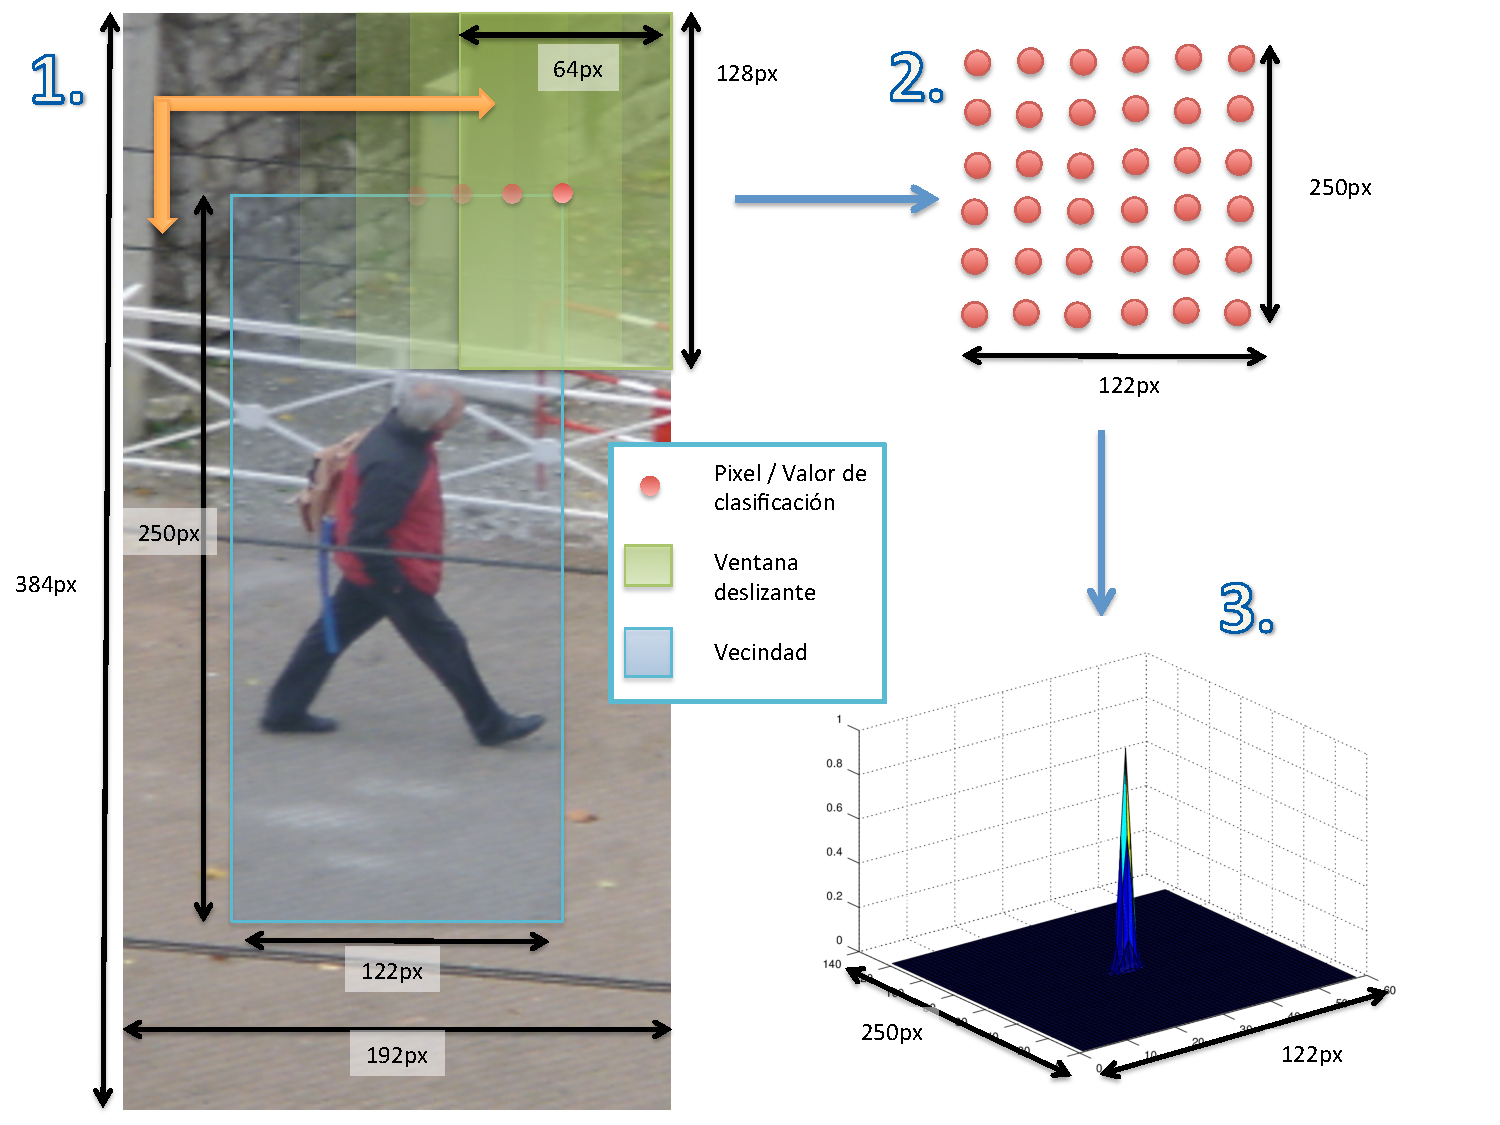
\includegraphics[scale=.6]{images/expected}
  \caption{\em Esquema de Proceso y Resultado esperado.}  
  \label{fig:expected}
\end{figure}

Por otra parte es esperable que un clasificador correctamente sintonizado (con un alta sensibilidad espacial) tenga una salida con mayor índice de confianza mientras la ventana de clasificación se encuentre más cerca del objeto a detectar y aun mucho mayor cuando se encuentre totalmente frente a este. Para comprender más fácilmente este efecto podemos observar en la fig~\ref{fig:expected} un esquema muy general del proceso por el cual se obtienen los resultados y cuales deberían ser los resultados esperados, en primer lugar se encuentra la ventana deslizante que realiza la detección píxel a píxel buscando un peatón en la imagen, luego los valores obtenidos son recogidos en una matriz y evaluados para obtener su gráfico el cual presenta el resultado esperado. Dado que la persona se encuentra en el centro de la imagen es de esperar que en esa zona la confianza de la decisión del clasificador sea mucho más alta que para el resto de la imagen y en un escenario teórico ideal esperamos que la respuesta sea un único impulso en el centro de la imagen analizada pues esto simplificaría de forma considerable el post-procesamiento.


\section{M\'etricas propuestas}
\label{metricas:propuestas}

La \cite{IEEE1990} define un métrica como ``Una medida cuantitativa del grado en que un sistema, componente o proceso posee un atributo dado'', por lo tanto el objetivo de la métrica debe ser en este caso particular definir el grado de sensibilidad espacial que poseen un clasificador para la detección de personas.

\subsection{Curtosis y Asimetría}
\label{propuestas:kys}

Inicialmente se consideró la utilización de una extensión a dos dimensiones de dos medidas que se utilizan en estadística y permitirían describir la sensibilidad espacial, estas son la curtosis (\textit{kurtosis}) y la asimetría (\textit{skewness}). Estas medidas aplicadas sobre los datos obtenidos entregan una descripción de la forma de la distribución. En el caso de la curtosis, mientras mayor sea su valor, la respuesta del clasificador representaría una concentración mayor de datos cercanos a la media, que coexisten con una frecuencia relativamente elevada de datos alejado de ésta. Por otro lado, la asimetría indicará cuán desplazada se encuentra la distribución de un centro de referencia simétrico. Específicamente la curtosis se mide utilizando el coeficiente de curtosis el cual tiene valor 3 cuando la distribución es de tipo normal o mesocúrtica, si el valor es mayor a 3 se conoce como distribución leptocúrtica y si el valor es menor que 3 la distribución es platicúrtica. En la figura~\ref{fig:curtosis} se puede observar de forma gráfica el fenómeno de la curtosis. 

\begin{figure}[tp]
  \centering
  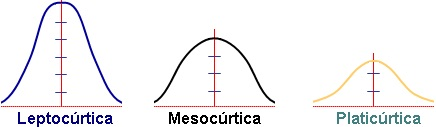
\includegraphics[scale=.6]{images/curtosis}
  \caption{\em Tipos de distribución según su valor de curtosis.}  
  \label{fig:curtosis}
\end{figure}

La asimetría se puede medir con el coeficiente de asimetría de Fisher. Cuando este coeficiente toma valores negativos la distribución es asimétrica negativa o está desplazada a la izquierda, mientras que si el valor es positivo, la distribución es asimétrica positiva y está desplazada a la derecha. En el caso de que la distribución sea simétrica, el valor del coeficiente es cero, sin embargo, el caso contrario no es siempre correcto. El desplazamiento de la asimetría se puede observar gráficamente en la figura~\ref{fig:asimetria}. 

\begin{figure}[tp]
  \centering
  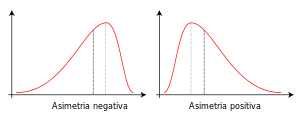
\includegraphics[scale=.6]{images/asimetria}
  \caption{\em Tipos de distribución según su valor de asimetría.}  
  \label{fig:asimetria}
\end{figure}

Estas medidas son muy útiles al trabajar con datos en una dimensión. Sin embargo al realizar una extensión de este procedimiento a dos dimensiones los resultados no fueron los esperados, por lo que fueron reemplazadas por un método más directo que permitiría determinar cuán malo es el valor de la sensibilidad espacial respecto de un modelo dado.

\subsection{Promedio ponderado de las diferencias (PPD)}

\begin{figure}[tp]
  \centering
  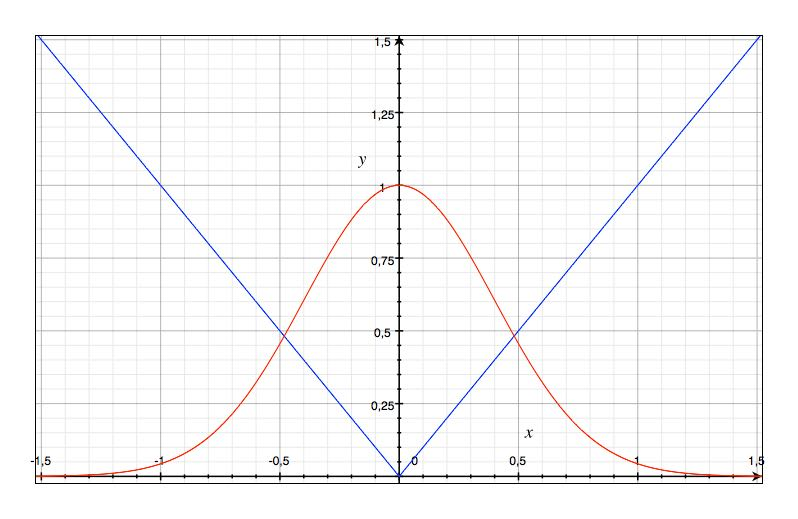
\includegraphics[scale=.4]{images/grafico_ppd}
  \caption{\em Representación de las funciones utilizadas para el cálculo del PPD.}  
  \label{fig:ppd}
\end{figure}

Dadas las dificultades encontradas utilizando la curtosis y la asimetría se hace necesario plantear un nuevo modelo de métrica que  permita describir de mejor forma la sensibilidad espacial. El nuevo modelo de sensibilidad espacial esta inspirado en una distribución normal, dado que en la práctica la probabilidad de obtener un resultado como un impulso es muy baja, por lo que el modelo normal se ajusta mejor a la realidad del fenómeno. La métrica propuesta evalúa el valor absoluto de las diferencias punto a punto de la matriz resultado respecto del modelo de distribución normal en tres dimensiones, luego realiza un promedio ponderado por una función cónica. En la figura~\ref{fig:ppd} se puede observar la abstracción del modelo en dos dimensiones. Es importante señalar que el set de datos se adaptó con una transformación en la cual se situó a la persona a detectar en el centro de la imagen de cada imagen de test y se estandarizó el tamaño de todas estas imágenes. De esta forma se puede comparar en mejor forma distintas combinaciones de descriptor/clasificador.

\begin{figure}[htc]
  \centering
  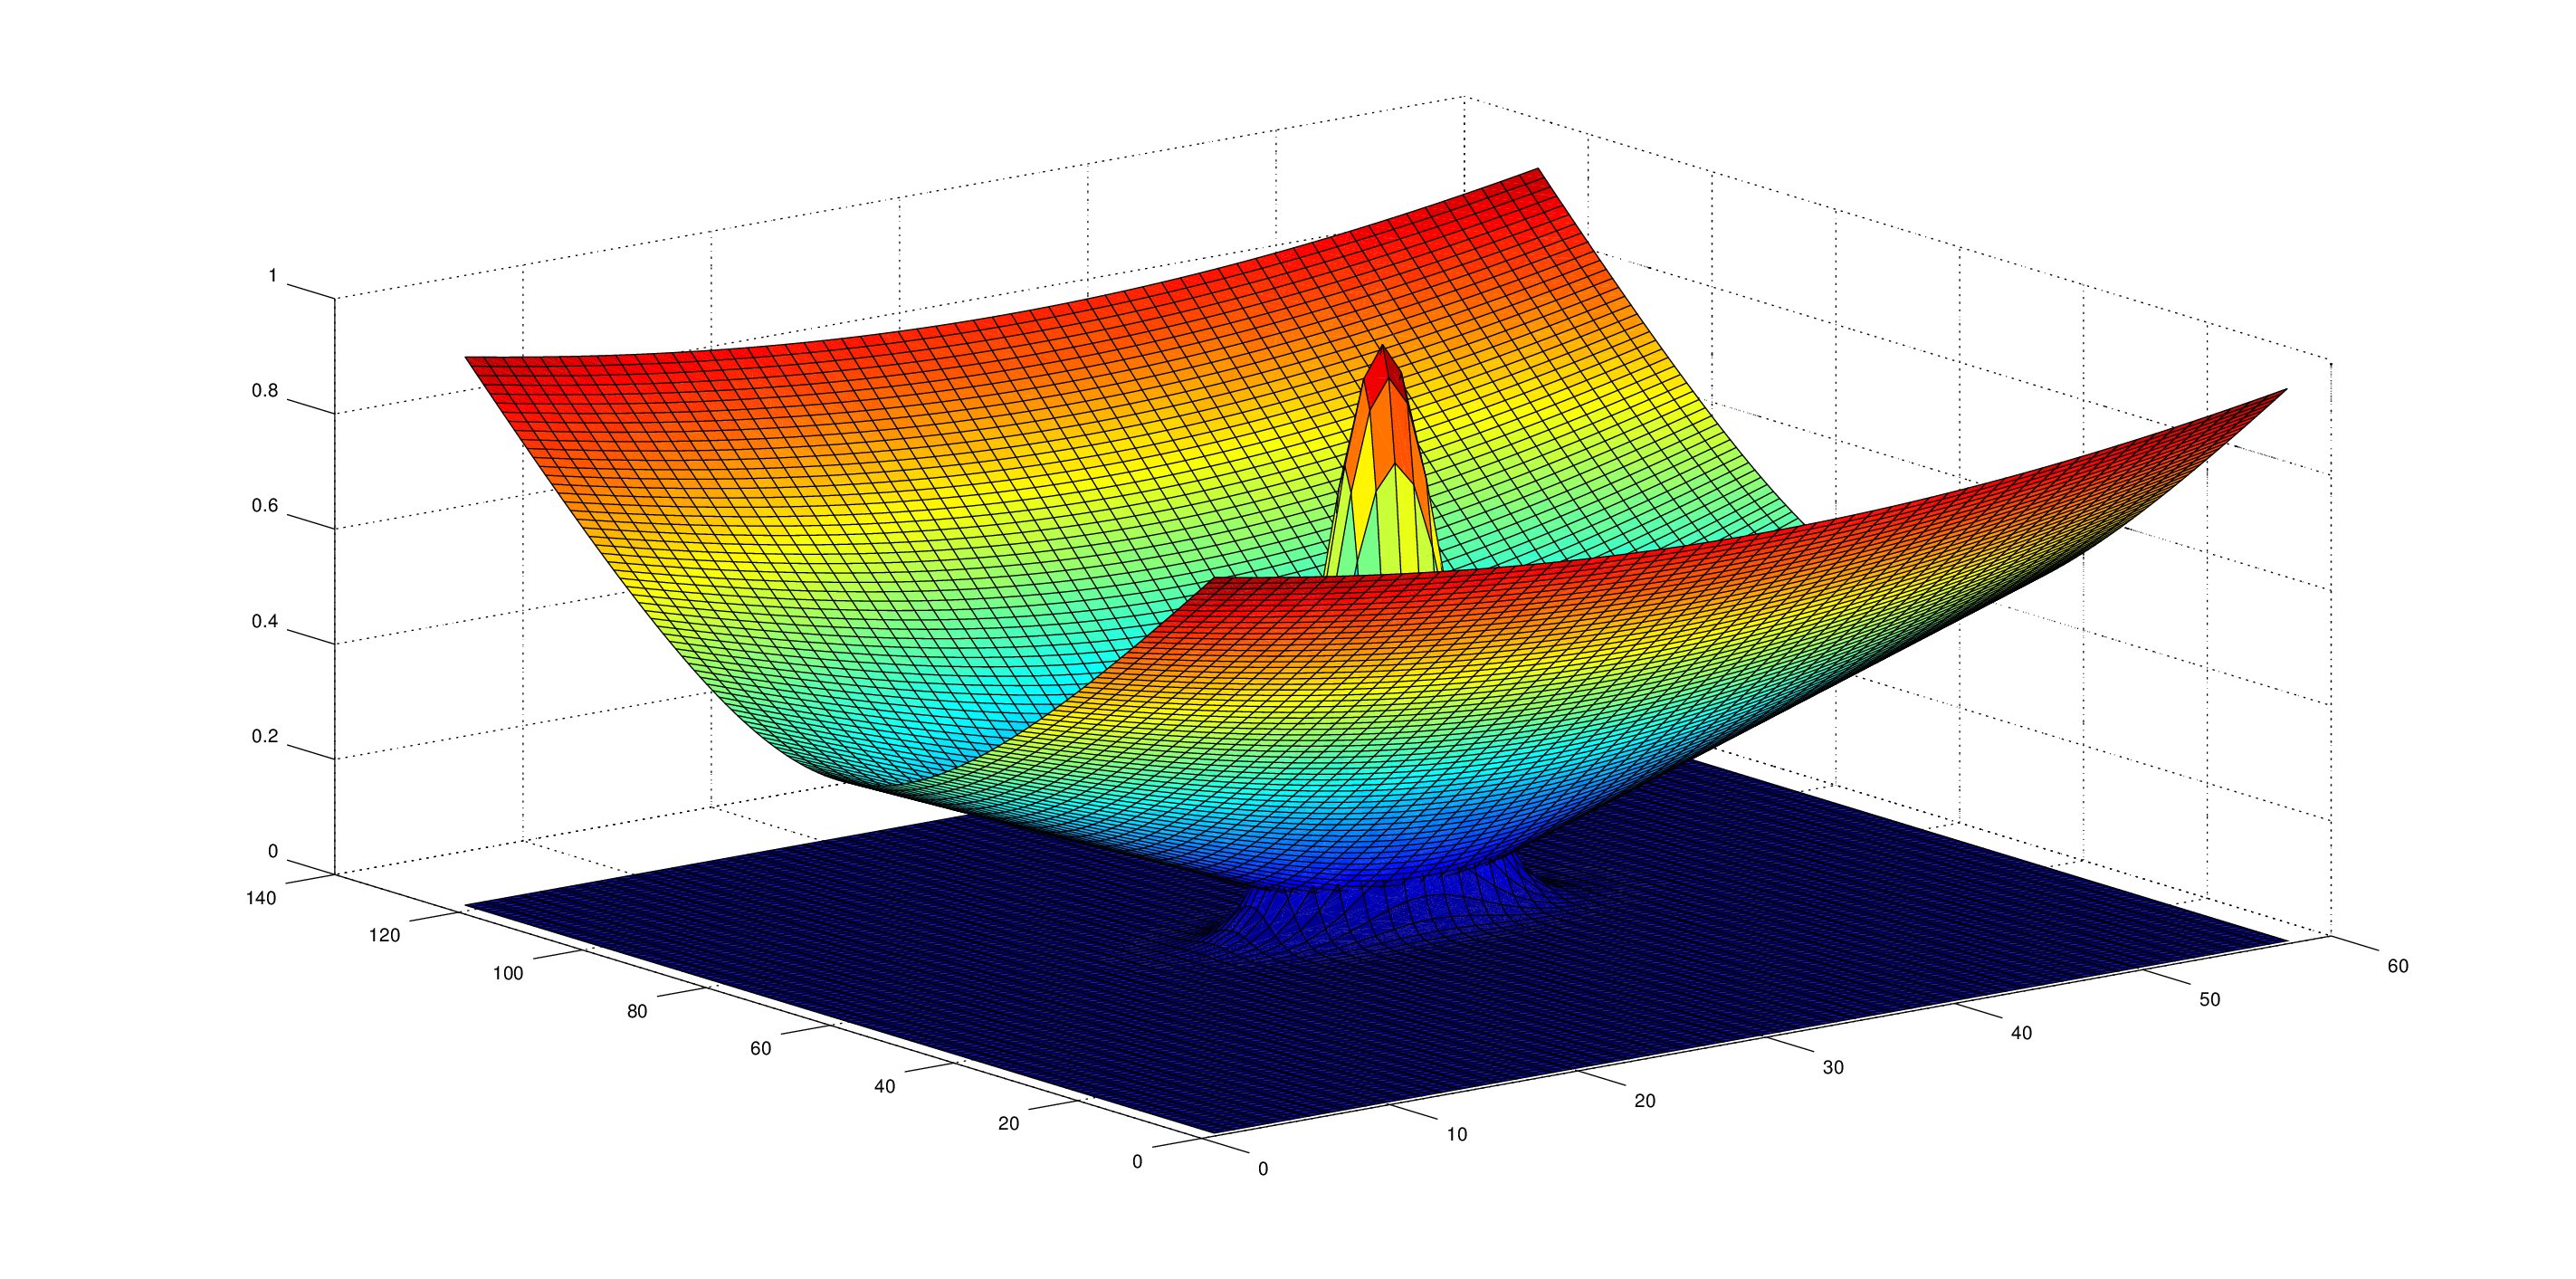
\includegraphics[scale=.3]{images/metrica}
  \caption{\em Representación en tres dimensiones de las funciones utilizadas para el cálculo del PPD.}  
  \label{fig:ppd3d}
\end{figure}

El modelo en tres dimensiones de la métrica es difícil de visualizar por la diferencia de tamaño entre la función cónica y la función normal, sin embargo, en la figura~\ref{fig:ppd3d} se realizó un ajuste de la escala para poder visualizar el efecto.

\subsubsection{Demostración matemática}
\label{sec:dem}

Para demostrar que la función aplicada PPD es efectivamente una métrica es necesario demostrar matemáticamente que cumple con las condiciones para serlo. A continuación se presenta la definición matemática de métrica y la demostración de que PPD cumple con dicha definición
noSea \textit{X} un conjunto. Una función \(d:X\times X\rightarrow \mathbb{R}\) se llama \textit{distancia o métrica} sobre \textit{X} si se cumplen los axiomas de métrica.

\begin{enumerate}
\item \(d(x,y)\geq\)~0
\item \(d(x,y) = \)~0~\(\Leftrightarrow x=y\)
\item \(d(x,y)=d(y,x)\)
\item \(d(x,z)\geq~d(x,y)+d(y,z)\)
\end{enumerate}

Luego de definir una métrica se da paso a la demostración. Sea \(z(x,y)\) la función resultado. Sea \(w(x,y)\) la función modelo. Sea \(c(x,y)\) la función cónica. Donde \(x = 0,1,...,m-1\) e \(y = 0,1,...,n-1\). Entonces la ponderación de la función resultado y modelo con la cónica se puede escribir como.

% ***SAV creo que es mejor no usar * (se confunde con otro operador como convolución) ***DQ Revisado

\begin{enumerate}
\item \(f(x,y) = z(x,y)\ c(x,y) = v_{k}\)
\item \(g(x,y) = w(x,y)\ c(x,y) = u_{k}\)
\end{enumerate}

Donde \(k = 0, 1, 2, ..., mn-1.\) la métrica propuesta queda definida por la expresión~\ref{eq:met}.

\begin{equation}
\centering
\label{eq:met}
 d(u_{k},v_{k})=\sum_{k=0}^{mn-1} \left | u_{k}- v_{k}\right |
\end{equation}

Evaluando los axiomas:
 

\begin{enumerate}
\item \(como \left | u_{k}- v_{k}\right | \geq~0 \forall~k \in~[0,nm-1)] \\ entonces  \sum_{k=0}^{m\ n-1} \left | u_{k}- v_{k}\right | \\ \therefore~d(u_{k},v_{k})\geq~0\)

\item \(d(u_{k},v_{k}) = 0 \\ \Rightarrow \sum_{k=0}^{mn-1} \left | u_{k}- v_{k}\right | = 0 \\ \Rightarrow  \left | u_{k}- v_{k}\right | = 0 \forall~k \in~[0,nm-1] \\ \Rightarrow  u_{k}- v_{k} = 0 \forall~k \in~[0,nm-1] \\ \Rightarrow  u_{k} = v_{k} \)

\item \(d(u_{k},v_{k})=\sum_{k=0}^{mn-1} \left | u_{k}- v_{k}\right | = \sum_{k=0}^{mn-1} \left | v_{k}- u_{k}\right | =  d(v_{k},u_{k}) \)

\item \( d(u_{k},s_{k})=\sum_{k=0}^{mn-1} \left | u_{k} - s_{k}\right | \\
\sum_{k=0}^{mn-1} \left | u_{k} - s_{k}\right | \leq \sum_{k=0}^{mn-1} \left | u_{k} - v_{k}\right | + \left | v_{k} - s_{k}\right | \\
= \sum_{k=0}^{mn-1} \left | u_{k} - v_{k}\right | + \sum_{k=0}^{mn-1} \left | v_{k} - s_{k}\right | \\
= d(u_{k},v_{k}) + d(v_{k},s_{k}) \)

\end{enumerate}


Una vez realizada la demostración las métricas consideras deben ser evaluadas para comprobar su correcto funcionamiento. 

\section{Evaluaci\'on preliminar de las m\'etricas propuestas}
\label{metricas:evaluacion}



\begin{figure}[htc]
  \centering
  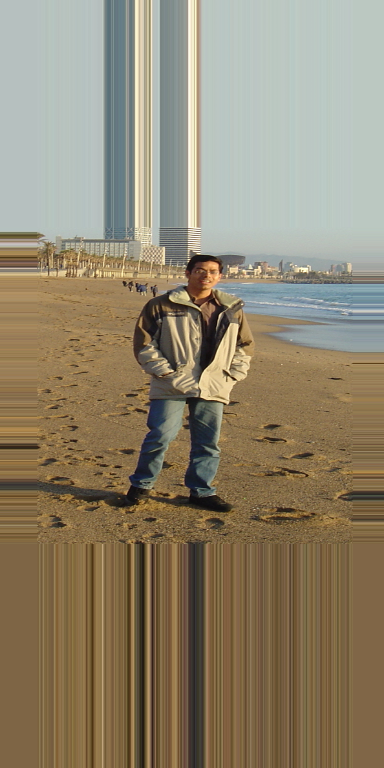
\includegraphics[scale=.25]{images/test1}
  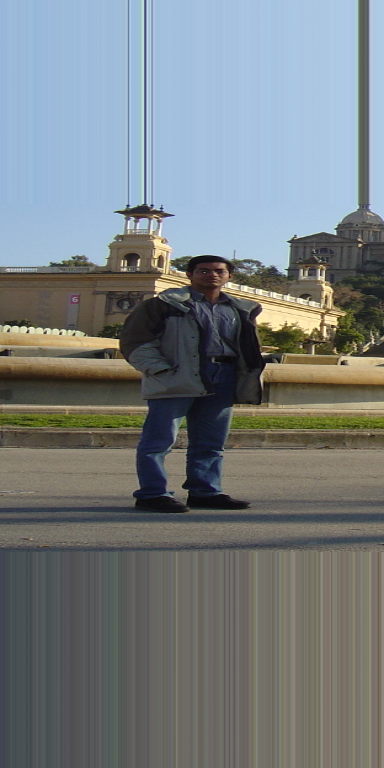
\includegraphics[scale=.25]{images/test2}
  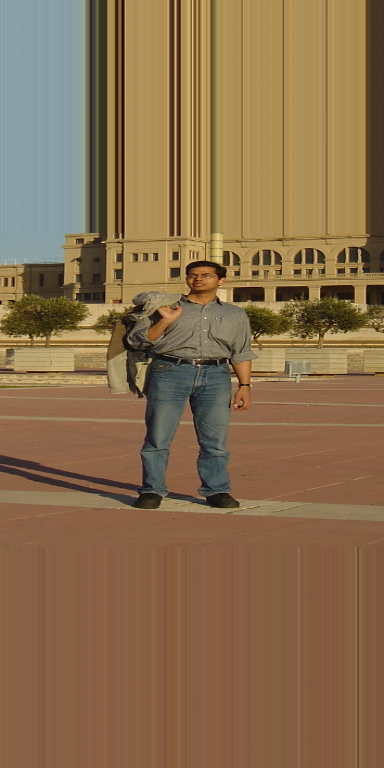
\includegraphics[scale=.25]{images/test3}
  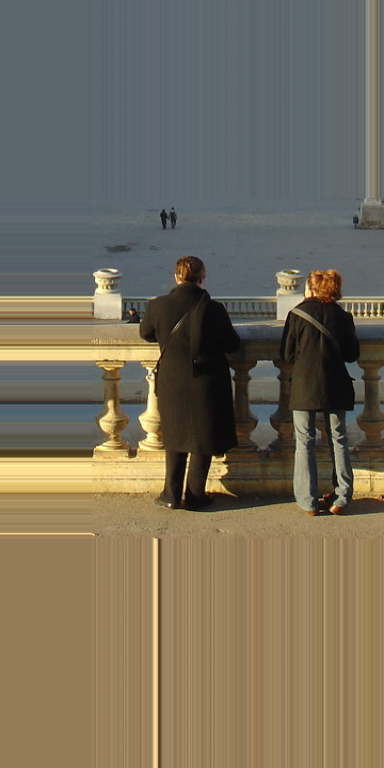
\includegraphics[scale=.25]{images/test4}
  \caption{\em Imágenes utilizadas en la evaluación preliminar, de izquierda a derecha test1.png, test2.png, test3.png, test4.png.}  
  \label{fig:testpersons}
\end{figure}

Una vez propuestas las métricas es necesario evaluar su contingencia respecto del problema de la sensibilidad espacial. Con este fin se desarrolló un software ejemplo preliminar que permite obtener una matriz resultado con valores correspondientes al grado de seguridad con la que un clasificador indica la existencia de un peatón alrededor del \textit{ground truth}. Para  esto se utilizó la implementación del detector utilizando HOG el cual está incluido dentro de la biblioteca OpenCV. Además se consideró como \textit{ground truth} el punto indicado en las anotaciones realizadas por Dalal que acompañan la descarga del set de datos INRIA. 
% ***SAV sería bueno poner una imagen ilustrando esto mostrando el peatón y la vecindad de análisis
Las imágenes utilizadas para realizar la evaluación preliminar fueron extraídas desde el mismo set de datos que finalmente sería utilizado para realizar el análisis comparativo. En la figura~\ref{fig:testpersons} se pueden revisar las imágenes utilizadas.

\begin{figure}[htc]
  \centering
  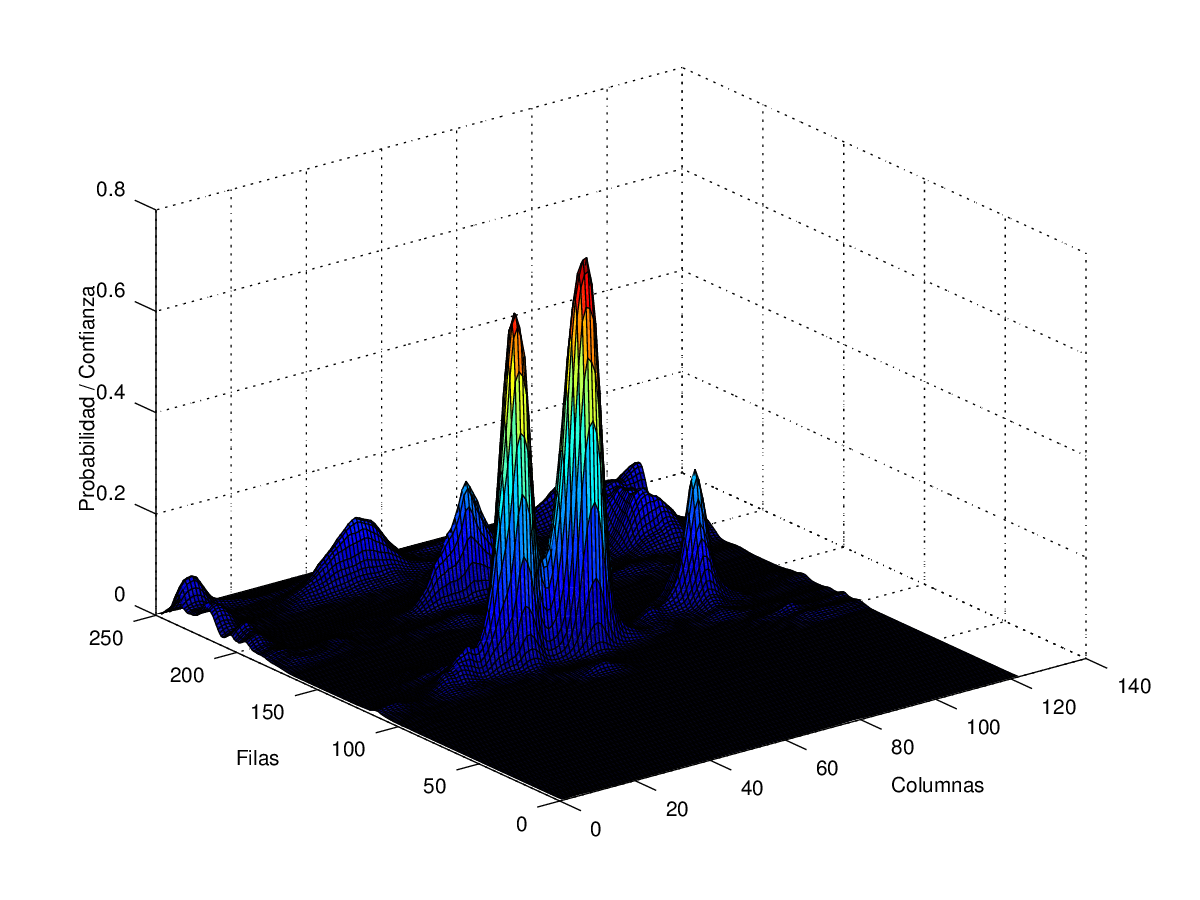
\includegraphics[scale=.6]{images/resultado_ejemplo}
  \caption{\em Resultado obtenido luego de realizar una clasificación exhaustiva de ``test1.png''}  
  \label{fig:ejemploresultado}
\end{figure}

% ***SAV son realmente 3 dimensiones? En el caso estandar es una dimension (por ejemplo el tiempo o una distancia lineal, y la "segunda" dimension es la respuesta). En ls imagenes son dos dimensiones x y más la respuesta. O sea la respuesta es una funcion de 2 dimensiones (x y). *** DQ revisado, efectivamente son dos dimensiones más la respuesta, solo el gráfico es en tres dimensiones.
Dados los problemas mencionados en la sección~\ref{propuestas:kys} sobre la extensión de las métricas a un espacio de dos dimensiones se realizaron las pruebas preliminares con las métricas de curtosis y asimetría para una dimensión, utilizando las proyecciones para las columnas y las filas. A continuación el proceso se detalla sólo para una de las imágenes (``test1.png'') y los resultados generales obtenidos (la gráfica del proceso completo se pueden encontrar en el Anexo~\ref{cap:gapm}).

\begin{figure}[htc]
  \centering
  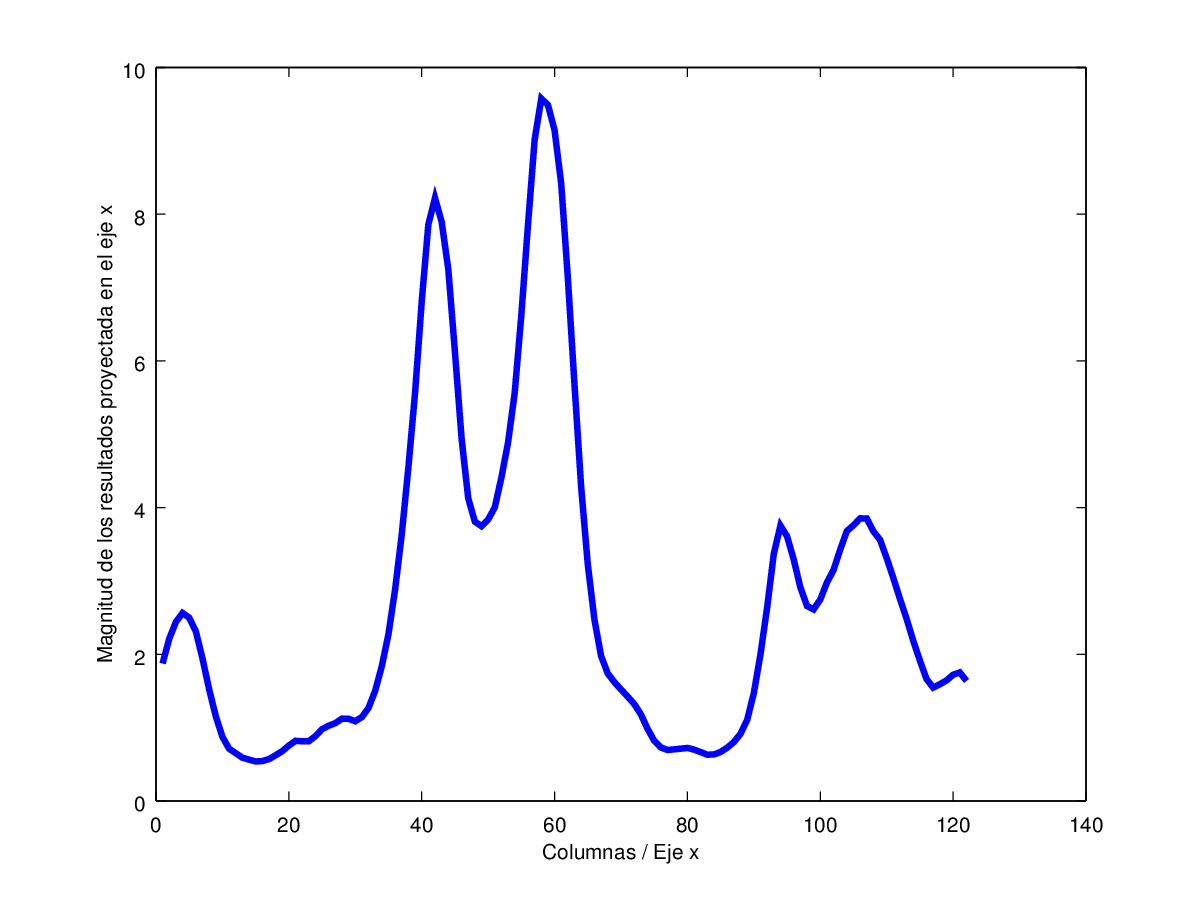
\includegraphics[scale=.35]{images/proyeccionx}
  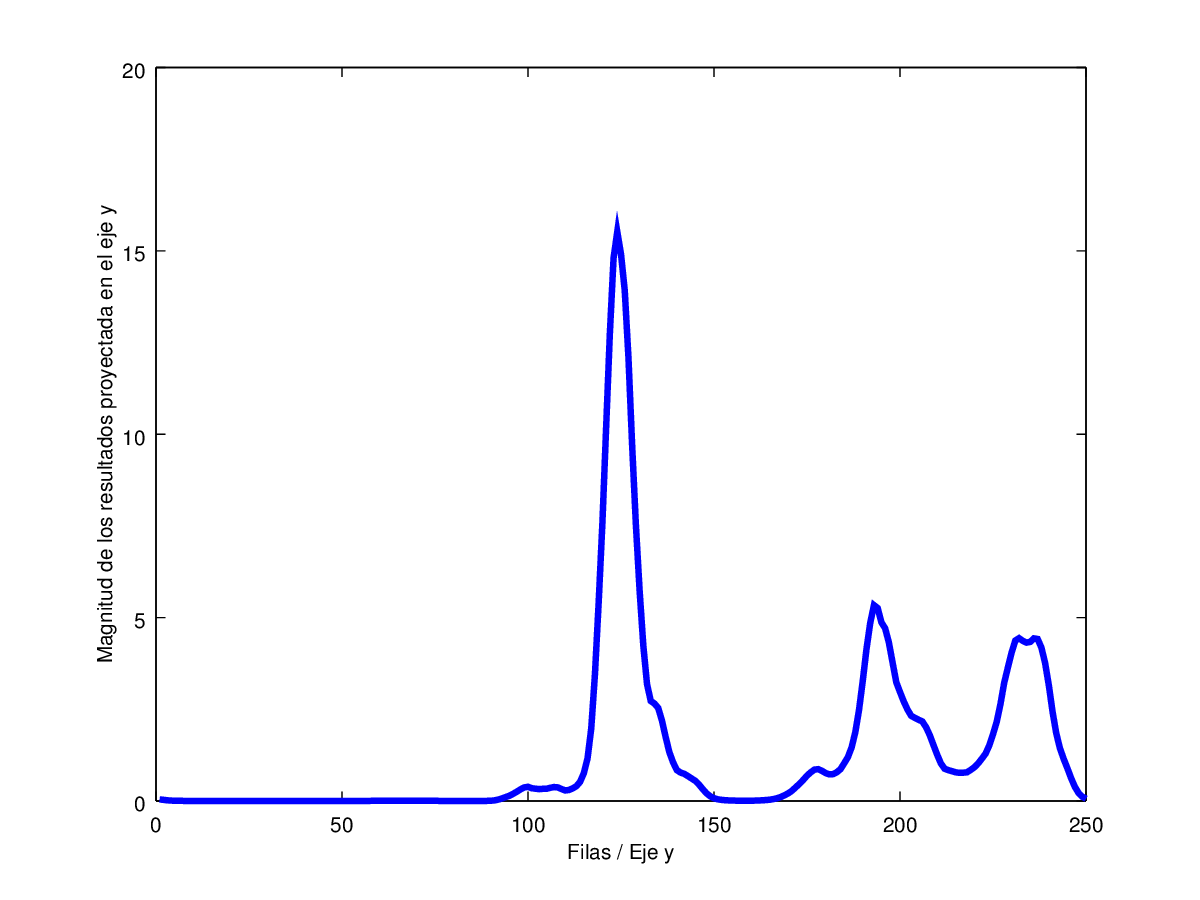
\includegraphics[scale=.35]{images/proyecciony}
  \caption{\em Proyección del resultado para los ejes x (izquierda) e y (derecha).}  
  \label{fig:proyecciones}
\end{figure}

Una vez realizada la clasificación exhaustiva en la imagen se obtiene un resultado como el de la figura~\ref{fig:ejemploresultado}, en este se pueden observar dos elevaciones bastante más pronunciadas que en el resto de la imagen, en la imagen hay solo una persona por lo que sería necesario utilizar NMS (non maximal suppression) para eliminar las detecciones múltiples. Analizaremos la posibilidad de caracterizar esto con la evaluación de la sensibilidad espacial. Para la realización de algunos de los cálculos es necesario obtener las proyecciones para el eje \textit{x} y para el eje \textit{y} las cuales se muestran en la figura~\ref{fig:proyecciones}.

Luego de la proyección, es preciso calcular el centroide y la desviación estándar cuyos valores son requisito previo para el cálculo de la curtosis y la asimetría, finalmente se realizó el cálculo de el PPD, el cual se aplica directamente sobre la matriz sin pasos intermedios, evaluando la diferencia de la matriz en cada punto con el modelo de función y ponderando posteriormente con la función cónica. Así se obtuvieron los resultados para las imágenes analizadas, estos resultados se muestran en la tabla~\ref{tab:resultadospreliminares}. A simple vista se puede comprobar que es posible calcular todas las métricas para todos los ejemplos.

\begin{table}[ht]
\centering
 \caption{\em Resultados obtenidos de la evaluación preliminar.}   \label{tab:resultadospreliminares}
\resizebox{15cm}{!} {
\begin{tabular}{c|c|c|c|c|c|c|c|c|c|}
\cline{2-10}
                                & Centroide x & Centroide y & \begin{tabular}[c]{@{}c@{}}Desviación\\  estándar x\end{tabular} & \begin{tabular}[c]{@{}c@{}}Desviación \\ estándar y\end{tabular} & Asimetría x & Asimetría y & Curtosis x & Curtosis y & PPD    \\ \hline
\multicolumn{1}{|c|}{test1.png} & 61,79       & 167,36      & 30,06                                                            & 46,46                                                            & 0,18        & 0,24        & 2,33       & 1,47       & 0.62338 \\ \hline
\multicolumn{1}{|c|}{test2.png} & 56,74       & 158,8       & 30,26                                                            & 41,74                                                            & 0,3         & 0,49        & 2.51       & 1,86       & 1.39056 \\ \hline
\multicolumn{1}{|c|}{test3.png} & 56,96       & 148,62      & 23,61                                                            & 43,17                                                            & 0,25        & 1,11        & 4,16       & 2,66       & 0.84709 \\ \hline
\multicolumn{1}{|c|}{test4.png} & 66,61       & 131,91      & 27,70                                                            & 40,85                                                            & 0,11        & 1,38        & 2,29       & 3,8        & 0.92963 \\ \hline
\end{tabular}}
\end{table}

Los valores de centroide, desviación estándar, asimetría y curtosis como se mencionó anteriormente son métricas que permiten realizar una descripción de la forma, podemos a través de ellas realizar un breve análisis. Conociendo ambos centroides podemos conocer la posición del centroide en el plano \textit{(x,y)}. Por otra parte la asimetría nos indica hacia donde se encuentra desplazada la distribución de valores, sin embargo no entregan mayor información en cuanto a que tan sensible o no es el comportamiento del clasificador. El PPD si bien no entrega información en detalle de la forma, indica de forma directa un valor representativo de sensibilidad espacial y se acerca mejor al objetivo de realizar una comparación ya que el indicador entrega un valor mayor mientras peor sea la sensibilidad del clasificador. Sin embargo, la métrica tiene algunos puntos ciegos, por ejemplo cuando el valor evaluado es cero el resultado es positivo  como se muestra en la tabla~\ref{tab:planas}. Esto resulta inconveniente para diferenciar de otra repuesta que tenga una diferencia semejante con el modelo planteado, pero en el sentido opuesto.

\begin{table}[htc]
\centering
  \caption{\em Evaluación de matrices con valores constantes para todos sus puntos. }   \label{tab:planas}
\begin{tabular}{c|c|}
\cline{2-2}
                                 & PPD    \\ \hline
\multicolumn{1}{|c|}{Matriz 0}   &  0.00000602 \\ \hline
\multicolumn{1}{|c|}{Matriz 0.1} &  0.73720 \\ \hline
\multicolumn{1}{|c|}{Matriz 0.5}  & 36.85977 \\ \hline
\multicolumn{1}{|c|}{Matriz 1}  &  73.71955 \\ \hline
\end{tabular}
\end{table}

Comprobando los resultados de las métricas se puede comprender que estas son complementarias y ambas son útiles, para caracterizar la sensibilidad espacial, sin embargo, dado su perfil comparativo, PPD es la mejor elección para continuar el análisis.

\section{Conclusiones del capítulo}
\label{metricas:conclusiones}

Resumiendo, en este capítulo se ha hablado acerca de las métricas, esto es, de las medidas cuantitativas del grado en que un sistema, componente o proceso posee un atributo dado. Las métricas a las que se hace mención son aquellas establecidas con respecto de la sensibilidad espacial de los clasificadores, esto es, cómo responde el clasificador a medida que la ventana de desplazamiento se va deslizando por la imagen, siendo el caso ideal que el clasificador no detectará ningún objeto válido (en este caso, personas) a menos que ésta se encuentre perfectamente centrada dentro de la ventana de detección, por lo que idealmente no debería detectar a una persona si sólo está contenida parcialmente dentro de la ventana de detección. A través del establecimiento de las métricas se puede determinar de manera concreta qué tan buena es la sensibilidad espacial de determinado clasificador, factor que constituye parte fundamental del presente trabajo. 

La sensibilidad espacial de un clasificador debe ser caracterizada para ayudar a mejorar el problema del post-procesamiento. Sin embargo, es necesario cuantificar este comportamiento; para esto se proponen en total tres métodos, dos de forma (curtosis y asimetría) y una de magnitud (PPD). Estas métricas son complementarias en el análisis y la caracterización de la sensibilidad espacial. Sin embargo, PPD es la mejor alternativa para la prosecución del presente trabajo, dado que permite realizar una comparación directa. Por otra parte, como trabajo futuro, es importante realizar aportes sobre las métricas tanto para mejorarlas como para complementar con otras que permitan un avance en la caracterización completa de la sensibilidad espacial.

En los capítulos siguientes se explicará en detalle el funcionamiento de los descriptores de características y clasificadores utilizados en el proceso.